%% ****** Start of file sortemplate.tex ****** %
%%
%%   This file is part of the files in the distribution of AIP substyles for REVTeX4.
%%   Version 4.2 of December 2014.
%%
%
% This is a template for producing documents for use with 
% the REVTEX 4.2 document class and the AIP substyles.
% 
% Copy this file to another name and then work on that file.
% That way, you always have this original template file to use.

\documentclass[apj,twocolumn]{openjournal}
\usepackage{amsmath}
%\usepackage{caption}
%\usepackage{subcaption}
\usepackage{booktabs}

%\usepackage{caption}

%\captionsetup[table]{
%    font={small},
%    labelfont={bf},
%    justification=justified, % or 'raggedright' for left alignment
%    singlelinecheck=false,
%}

\usepackage[dvipsnames]{xcolor} %added later for color
\usepackage[breaklinks,colorlinks,citecolor=blue,urlcolor=blue,linkcolor=blue]{hyperref}
%
%\newcommand{\norm}[1]{\left\lVert#1\right\rVert}
%
%\newcommand{\red}[1]{\textcolor{red}{#1}}
%\newcommand{\green}[1]{\textcolor{green}{#1}}
%\newcommand{\blue}[1]{\textcolor{blue}{#1}}



\usepackage{orcidlink}
\usepackage{subfigure}

\renewcommand{\arraystretch}{1.2}  
\setlength\tabcolsep{0.15cm}

\usepackage{listings}
\usepackage{color}

\usepackage{soul}
\usepackage{amsmath}
\usepackage{xspace}
\usepackage{graphicx}
\usepackage{enumitem}
\usepackage{amssymb}
\usepackage{xifthen}
\usepackage{hyperref}
\usepackage[normalem]{ulem}
\usepackage{multirow}
%\usepackage{lineno}
%\linenumbers

% remove indents in footnotes
\usepackage[hang,flushmargin]{footmisc} 

\usepackage{styles/todo_notes}
\usepackage{styles/abbreviations}

\newcommand{\placeholder}[1]{{\color{gray} \lipsum[#1]}}
\newcommand{\paraOutlineHdr}[1]{{\color{gray}[\textit{#1}]}}

% custom function for adding units
\makeatletter
\newcommand{\unit}[1]{%
    \,\mathrm{#1}\checknextarg}
\newcommand{\checknextarg}{\@ifnextchar\bgroup{\gobblenextarg}{}}
\newcommand{\gobblenextarg}[1]{\,\mathrm{#1}\@ifnextchar\bgroup{\gobblenextarg}{}}
\makeatother

% shorthands


\newif\ifstartedinmathmode
\newcommand{\msun}{%
  \relax\ifmmode\startedinmathmodetrue\else\startedinmathmodefalse\fi
  {\ifstartedinmathmode\unit{M_{\odot}}\else$\unit{M_{\odot}}$\fi}\xspace%
}

\newif\ifstartedinmathmode
\newcommand{\rsun}{%
  \relax\ifmmode\startedinmathmodetrue\else\startedinmathmodefalse\fi
  {\ifstartedinmathmode\unit{R_{\odot}}\else$\unit{R_{\odot}}$\fi}\xspace%
}

% Fix revtex/openjournal small-caps centered table captions...
\makeatletter
\renewcommand\@makecaption[2]{%
  \par
  \vskip\abovecaptionskip
  \begingroup
    \footnotesize\rmfamily
    \begingroup
      \samepage
      \flushing
      \let\footnote\@footnotemark@gobble
      \ifnum\pdfstrcmp{\@captype}{table}=0
        \@make@capt@title{\textsc{Table \thetable}}{#2}%
      \else
        \ifnum\pdfstrcmp{\@captype}{figure}=0
          \@make@capt@title{\textsc{Figure \thefigure}}{#2}%
        \else
          \@make@capt@title{#1}{#2}%
        \fi
      \fi\par
    \endgroup
  \endgroup
  \vskip\belowcaptionskip
}
\makeatother

\defcitealias{Kiel+2009:2009MNRAS.395.2326K}{KH09}


\begin{document}

\author{Tom Wagg\,\orcidlink{0000-0001-6147-5761}$^{1}$}
\author{Mathieu Renzo\,\orcidlink{0000-0002-6718-9472}$^{2}$}
\author{Katelyn Breivik\,\orcidlink{0000-0001-5228-6598}$^{3}$}
\author{David~D.~Hendriks\,\orcidlink{0000-0003-0872-7098}$^{4}$}


\affiliation{$^1$Department of Astronomy, University of Washington, Seattle, WA, 98195}
\affiliation{$^2$McWilliams Center for Cosmology and Astrophysics, Department of Physics, Carnegie Mellon University, Pittsburgh, PA 15213, USA}
\affiliation{$^3$University of Arizona, Department of Astronomy \& Steward Observatory, 933 N. Cherry Ave., Tucson, AZ 85721, USA}
\affiliation{$^4$Department of Physics, University of Surrey, Guildford GU2 7XH, Surrey, UK}

\email{Corresponding author: tomjwagg@gmail.com}
\title{Comparison of stellar companion ejection velocities from binaries\\evolved in different population synthesis codes}


\begin{abstract}
    We present a comparison of the predicted ejection velocities of disrupted binary companions in three different population synthesis codes: \cosmic, \compas and \binc, which use two independent algorithms. We confirm that, despite the codes producing different pre-supernova orbital evolution from the same initial conditions, they each find the ejection velocities of secondary stars from disrupted binaries are narrowly distributed about their pre-supernova orbital velocity. We additionally include a correction to the derivation included in \citet{Kiel+2009:2009MNRAS.395.2326K} that brings it into agreement with methods from other works for determining post-supernova binary orbital parameters. During this comparison we identified and resolved bugs in the kick prescriptions of \textit{all three} codes we considered, highlighting how open-science practices and code comparisons are essential for addressing implementation issues.
\end{abstract}

\maketitle
\section{Introduction}

Observations of pulsars in the Milky Way necessitate that they have a high velocity dispersion and hence that these objects acquire high velocities upon formation \citep[e.g.,][]{Gunn+1970:1970ApJ...160..979G, Hobbs+2005:2005MNRAS.360..974H, Igoshev+2020}. For compact objects formed via isolated binary evolution, these velocities are expected to be imparted at the moment of core-collapse. Even for a symmetric explosion, the instantaneous mass loss from a supernova (SN) changes the post-SN orbital parameters \citep{Blaauw+1961, Boersma+1961}. This is typically insufficient to disrupt the orbit, since the ejecta mass is often limited by loss during previous mass transfer phases, but in some cases (${\sim}16\%$) mass loss can unbind the binary and result in both binary constituents being ejected with their pre-SN orbital velocity \citep{Renzo+2019:2019A&A...624A..66R}. Moreover, asymmetry in the explosion can impart a significant natal kick on the newly formed compact object \citep[e.g.,][]{Shklovskii+1970:1970SvA....13..562S,Lyne+1994:1994Natur.369..127L,Janka+2013:2013MNRAS.434.1355J,Janka+2017:2017ApJ...837...84J}, which in the majority of cases is strong enough to disrupt a binary \citep[e.g.,][]{Renzo+2019:2019A&A...624A..66R}. Similar asymmetry in neutrino emission can result in additional natal kicks, which can dominate in the case of full fallback \citep[e.g.,][]{Janka+1994:1994A&A...290..496J,Burrows+1996:1996PhRvL..76..352B,Scheck+2006:2006A&A...457..963S,Wongwathanarat+2013,Coleman+2022:2022MNRAS.517.3938C,Vigna-Gomez+2024:2024PhRvL.132s1403V}.

The impact of these SNe kicks on the post-SN orbital parameters of a binary system has been considered in detail by many previous works \citep{Flannery+1975:1975A&A....39...61F,Sutantyo+1978:1978Ap&SS..54..479S,Hills+1983:1983ApJ...267..322H,Dewey+1987:1987ApJ...321..780D,Wijers+1992:1992A&A...261..145W,Brandt+1995:1995MNRAS.274..461B,Kalogera+1996:1996ApJ...471..352K,Tauris+1998:1998AA...330.1047T,Hurley+2002,Pfahl+2002,Belczynski+2008:2008ApJS..174..223B,Kiel+2009:2009MNRAS.395.2326K}. These investigations account for a variety of effects, with the most extensive handling eccentric pre-SN systems, including the effect of instantaneous symmetric mass loss, the impact of the natal kick on both the compact object and disruption of the system, the SN blast wave impulse on the secondary star and collisions between the compact object and star. For a detailed derivation, which explains how each of these effects impacts a binary in clear and compact vector notation, we refer the reader to Appendix B of \citet{Pfahl+2002}.

Binary stellar population synthesis codes apply different choices of these SN kick methodologies in their evolution. These difference have the potential to significantly change the subsequent evolution of binary systems after a SN. The post-SN eccentricity, semi-major axis and centre-of-mass velocity of bound systems, as well as rate of unbinding and ejection velocities of stars and compact objects, are sensitive to kick prescriptions. The impact on population synthesis predictions is therefore wide-ranging, for both bound (such as X-ray binaries and gravitational-wave sources) and unbound (such as runaway stars) binary products. In this paper we focus on how the ejections velocities of stellar companions compare for a binary with identical initial conditions evolved in different codes.

\section{Secondary ejection velocity comparisons}\label{sec:compare}

In this Section we compare the ejection velocities for secondary stars as calculated by different population synthesis codes. The \cosmic population synthesis code \citep{COSMIC} applies the method from \citet{Pfahl+2002} (though previously followed \citet{Kiel+2009:2009MNRAS.395.2326K}, see Section~\ref{sec:kiel}). Similarly, \compas \citep{COMPAS, Compas+2022:2022JOSS....7.3838C} uses the method of \citet{Pfahl+2002}. In contrast, \binc \citep{Izzard+2004:2004MNRAS.350..407I, Izzard+2006:2006A&A...460..565I, Izzard+2009:2009A&A...508.1359I, Izzard+2018:2018MNRAS.473.2984I, Izzard+2023:2023MNRAS.521...35I} applies \citet{Tauris+1998:1998AA...330.1047T}. The combination of these codes therefore allows us to cross-validate three implementations of two different algorithms for determining secondary ejection velocities.

\begin{table}[htb]
    \centering
    \begin{tabular}{c|l}
        \hline
        \hline
        Code & Supernova kick prescription \\
        \hline
        \multirow{2}{*}{\cosmic} & \citealt{Kiel+2009:2009MNRAS.395.2326K} ($<$v3.5.0) \\
         & \citealt{Pfahl+2002} ($\ge$v3.5.0) \\
        \compas & \citealt{Pfahl+2002}\\
        \binc & \citealt{Tauris+1998:1998AA...330.1047T}
    \end{tabular}
    \caption{The prescription for supernova natal kicks used in the population synthesis codes we consider.}
    \label{tab:kick-prescriptions}
\end{table}

\subsection{Initial conditions and pre-supernova evolution}

We evolve a representative mass-transferring massive binary with a range of random supernova natal kicks in each code. This binary has the following initial conditions: primary mass, $m_1 = 20 \msun$, secondary mass $m_2 = 15 \msun$, orbital period, $P = 100 \unit{days}$, eccentricity, $e = 0$, and metallicity, $Z = 0.02$. This system is representative of O-type stars that undergo case B mass transfer, which often produce ejected secondaries. We repeat the evolution 50,000 times, each with a different random natal kick magnitude and direction. For each code we draw natal kick magnitudes from a Maxwellian with $\sigma = 265 \unit{km}{s^{-1}}$ and apply the \citet{Fryer+2012:2012ApJ...749...91F} delayed remnant mass prescription, but otherwise use the code's default settings.

\begin{figure}
    \centering
    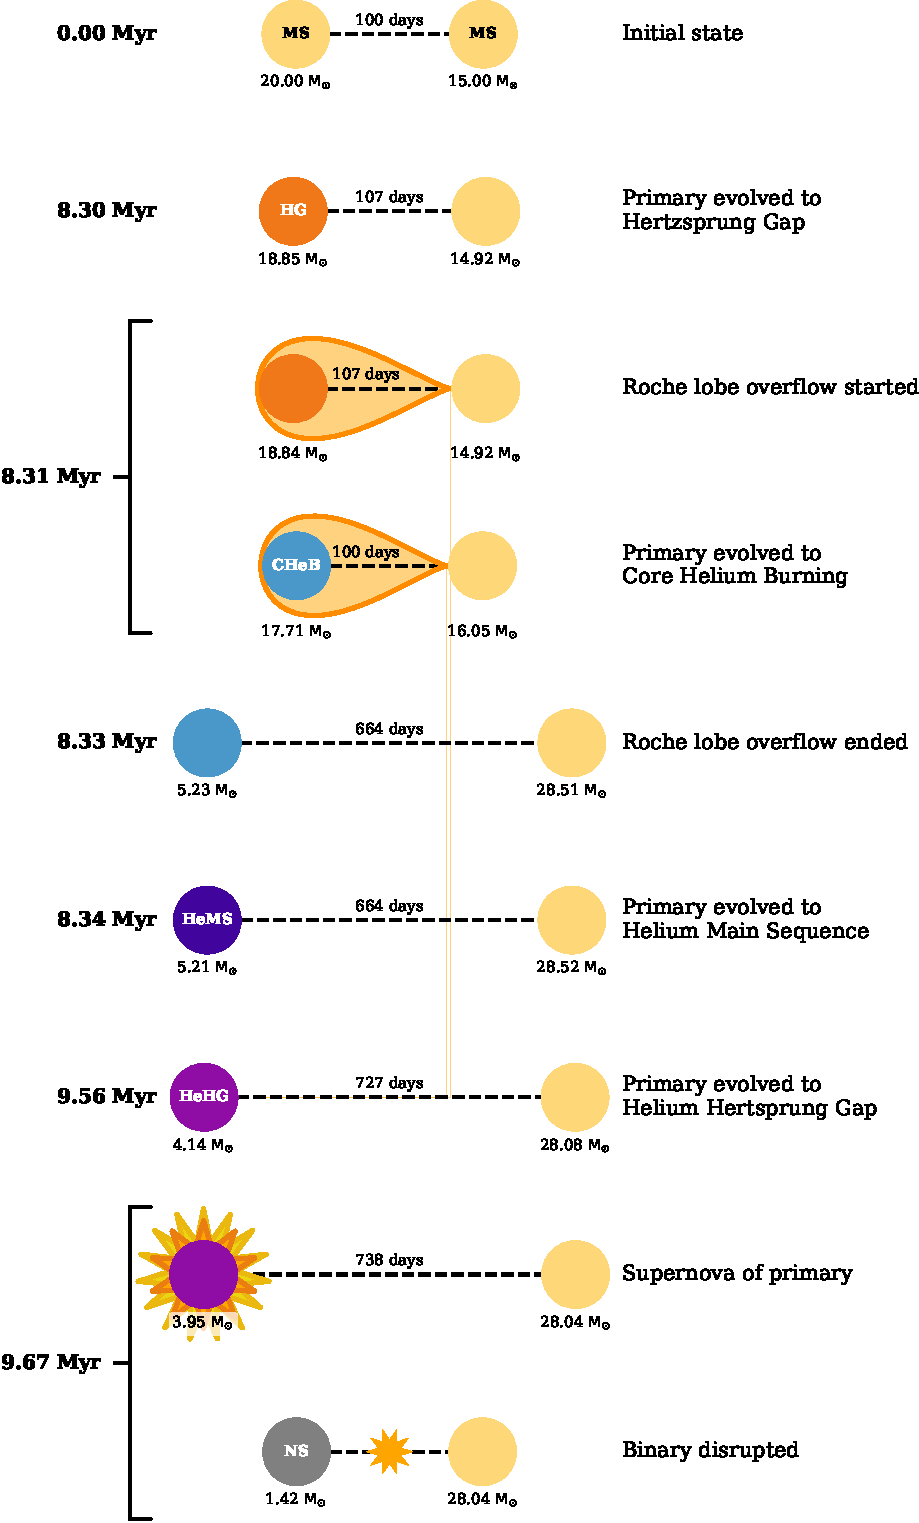
\includegraphics[width=\columnwidth]{figures/example_evolution.pdf}
    \caption{A cartoon evolution diagram of the representative binary that we consider. Each star is represented by a circle, where the colour represents the stellar type and their separation is scaled by their orbital period. Each row indicates an important timestep, which is labelled with its time and a description to the sides. Figure dynamically generated with \texttt{cogsworth} \citep{cogsworth_joss, cogsworth}}
    \label{fig:cartoon-evolution}
\end{figure}

The typical evolution of the system is to initiate stable case B mass transfer and unbind after the primary supernova.  In \cosmic, the primary star initiates almost fully-conservative mass transfer after $8.3\unit{Myr}$, as its expands on the Hertzprung gap. This transfers $13.6\unit{M_\odot}$ to the secondary star and widens the orbital period from ${\sim}100\unit{d}$ to ${\sim}660\unit{d}$. The primary proceeds to self-strip via stellar winds, further widening the binary until it reaches core collapse $1.5\unit{Myr}$ later.

The difference in binary physics settings between the codes results in moderately different pre-SN evolutionary states. In \compas the evolution proceeds similarly, except the mass transfer is much less conservative, such that a large fraction of the transferred mass is lost from the system. As a result, the companion is less massive (${\sim}18\unit{M_\odot}$) and the binary is wider (${\sim}800\unit{d}$) due to the angular-momentum loss from the system.
\david{Could you let me know how this roughly proceeds in \binc?}
It may be possible enforce agreement between codes through a detailed selection of binary physics settings but that is beyond the scope of this work.

\subsection{Ejection velocities}

\begin{figure*}[htb]
    \centering
    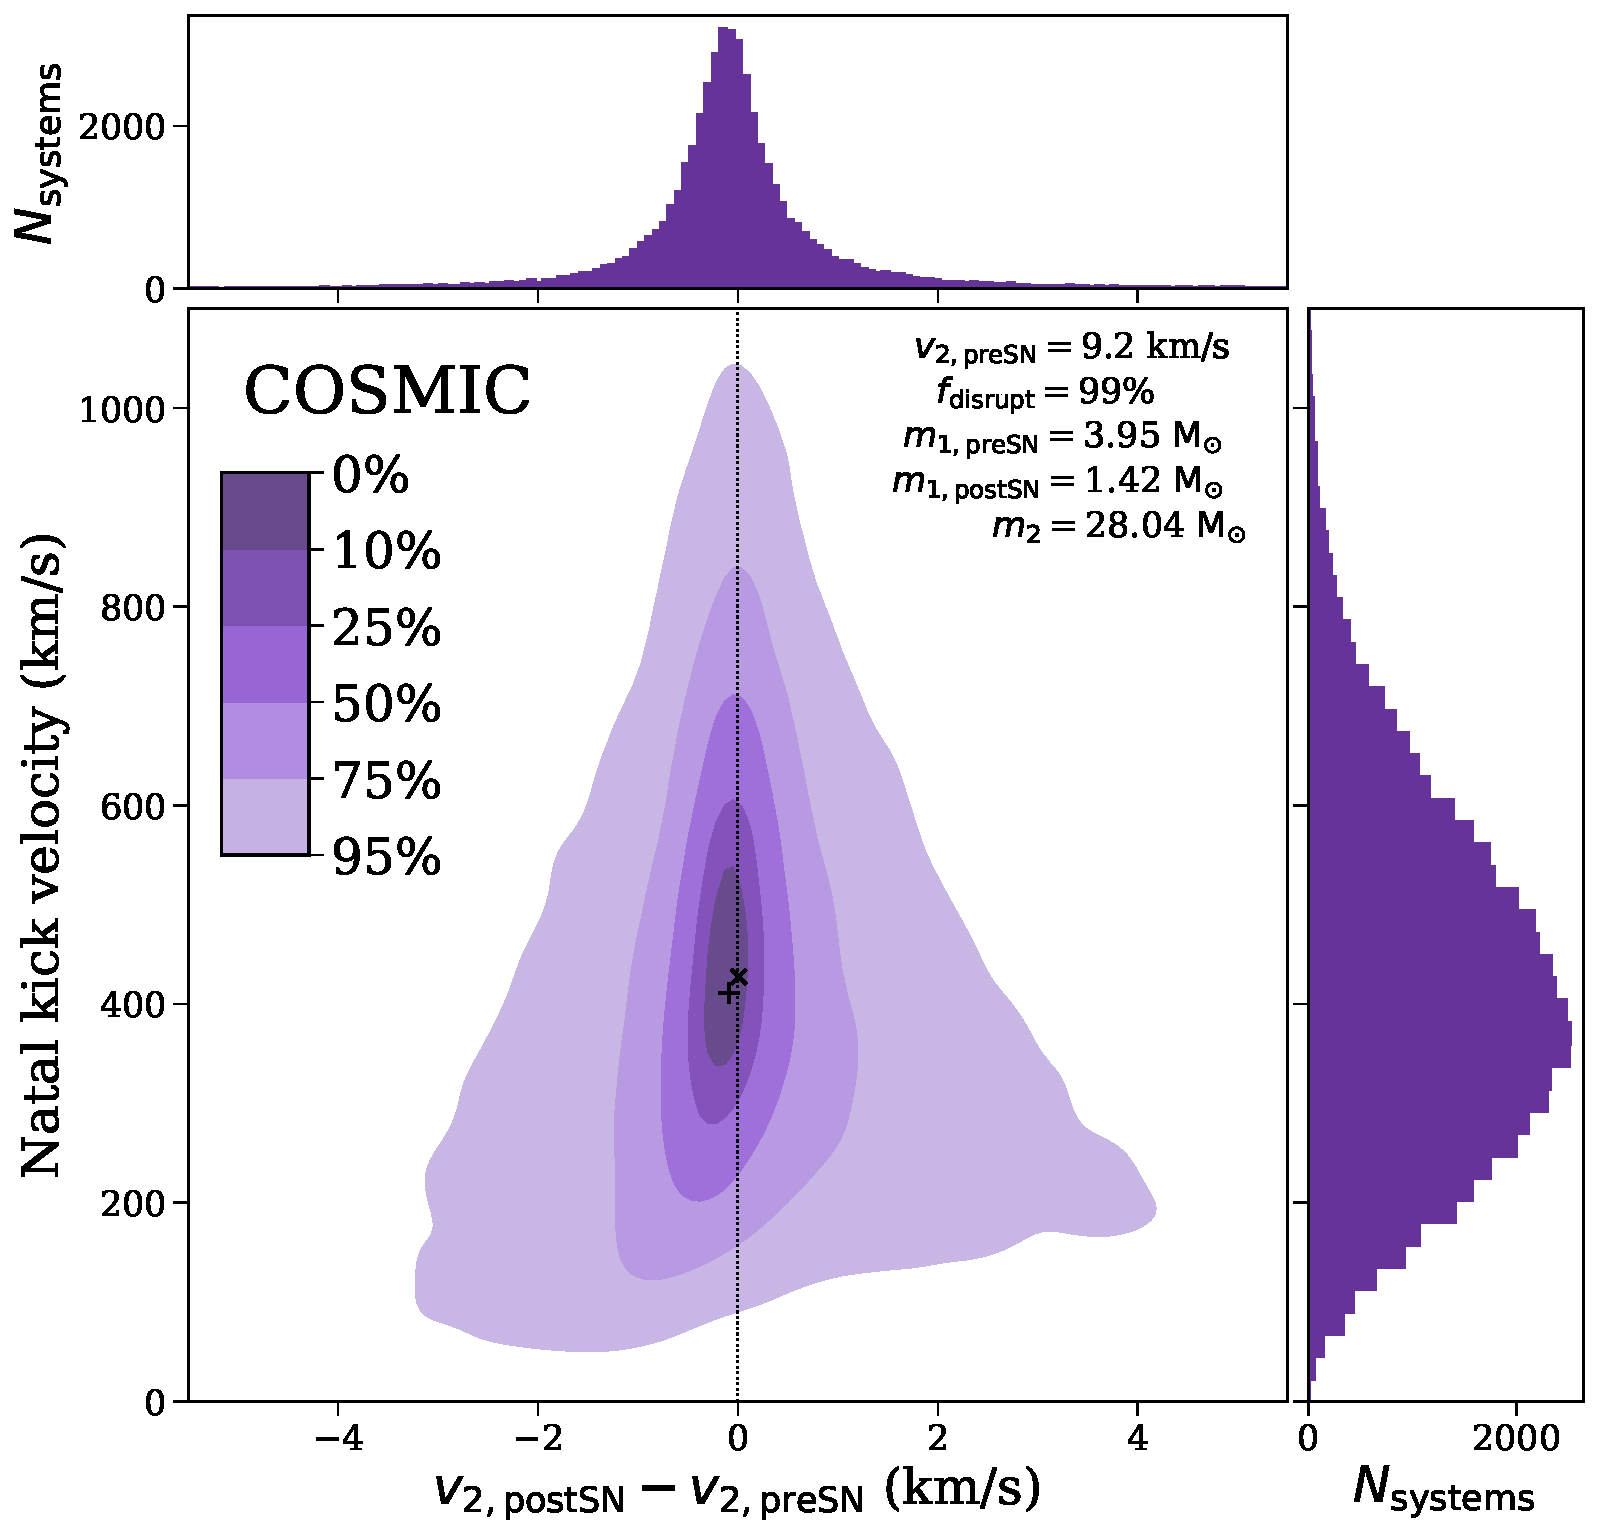
\includegraphics[width=0.45\textwidth]{figures/cosmic.pdf}
    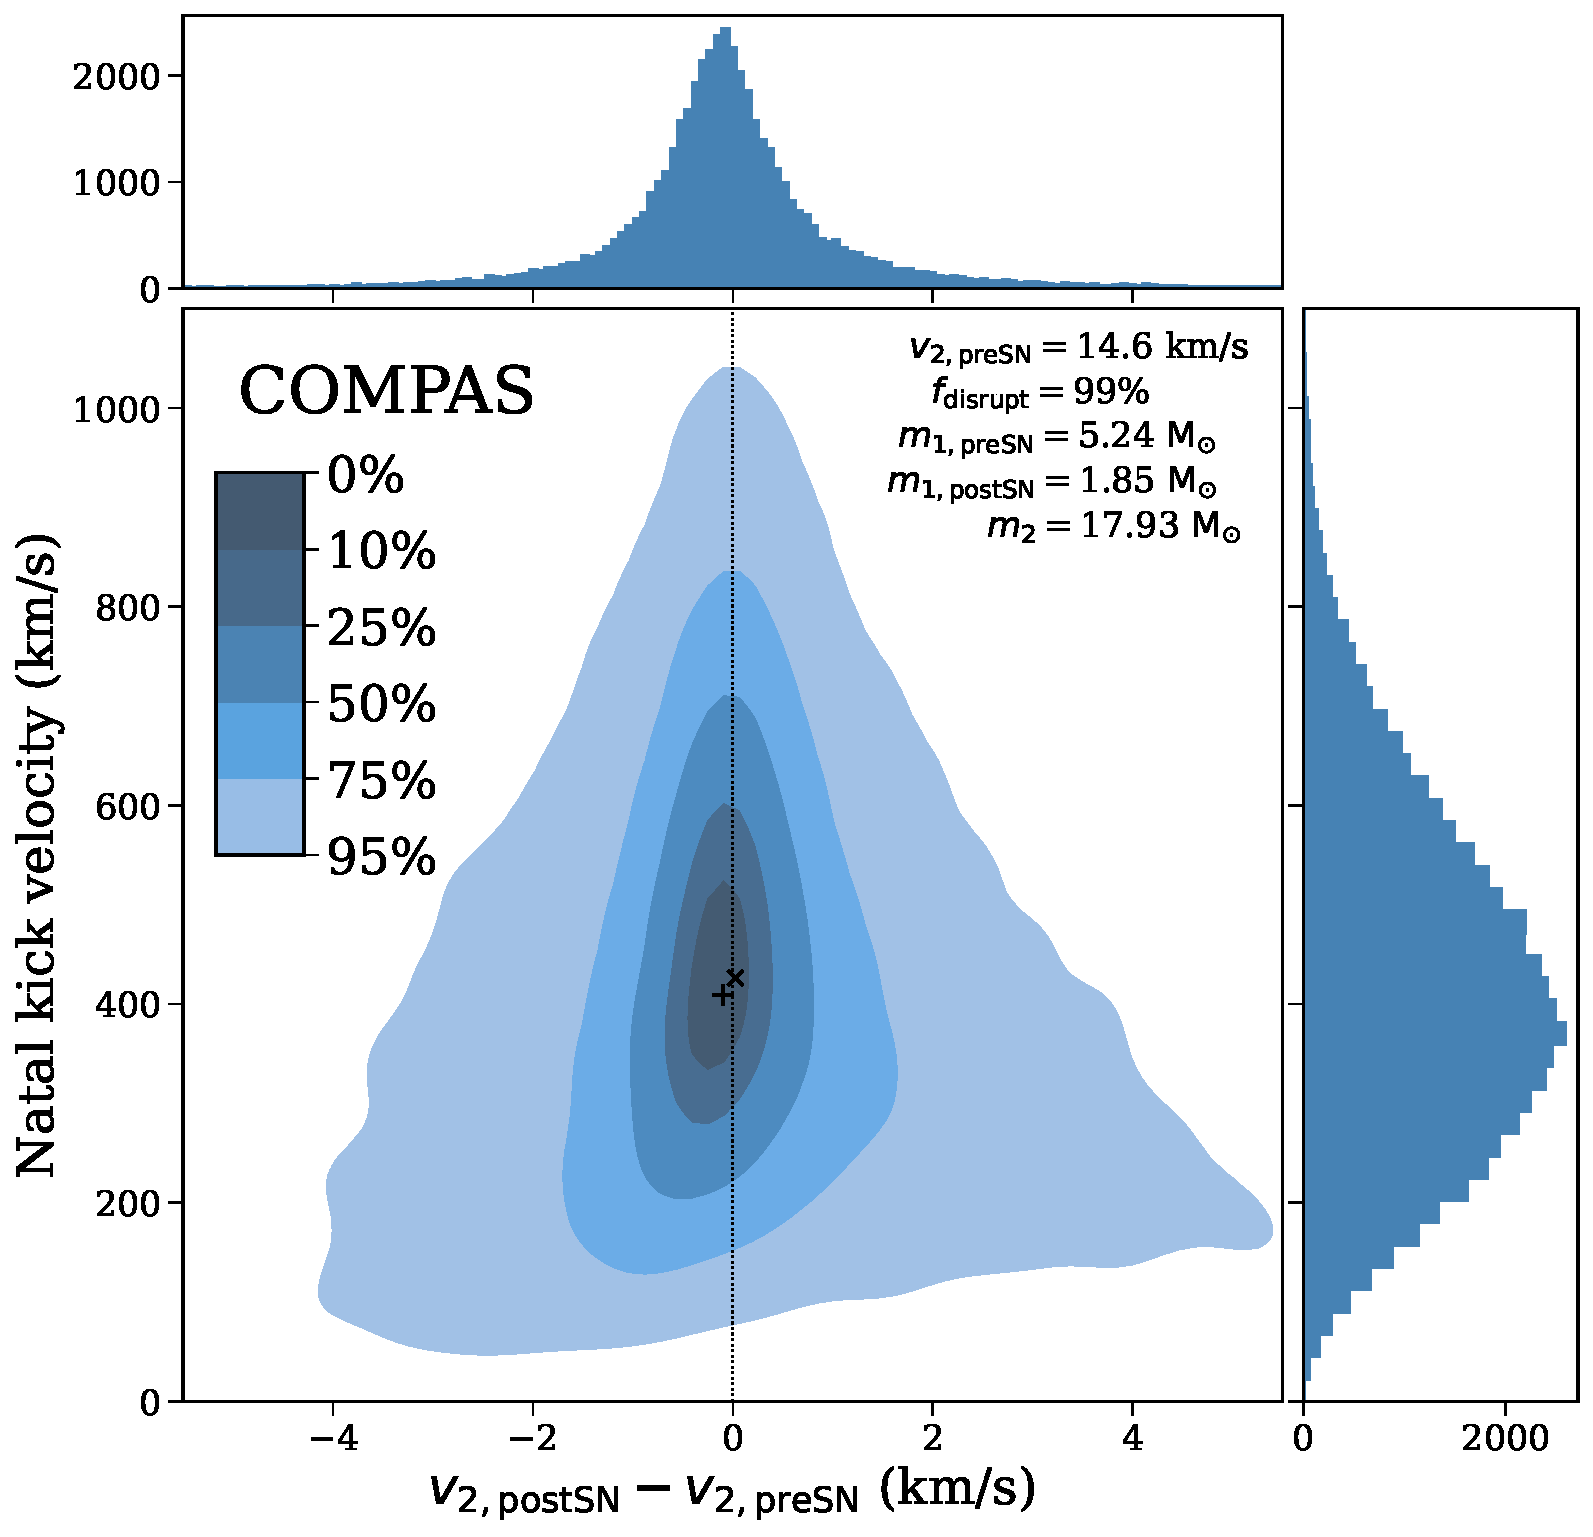
\includegraphics[width=0.45\textwidth]{figures/compas.pdf}
    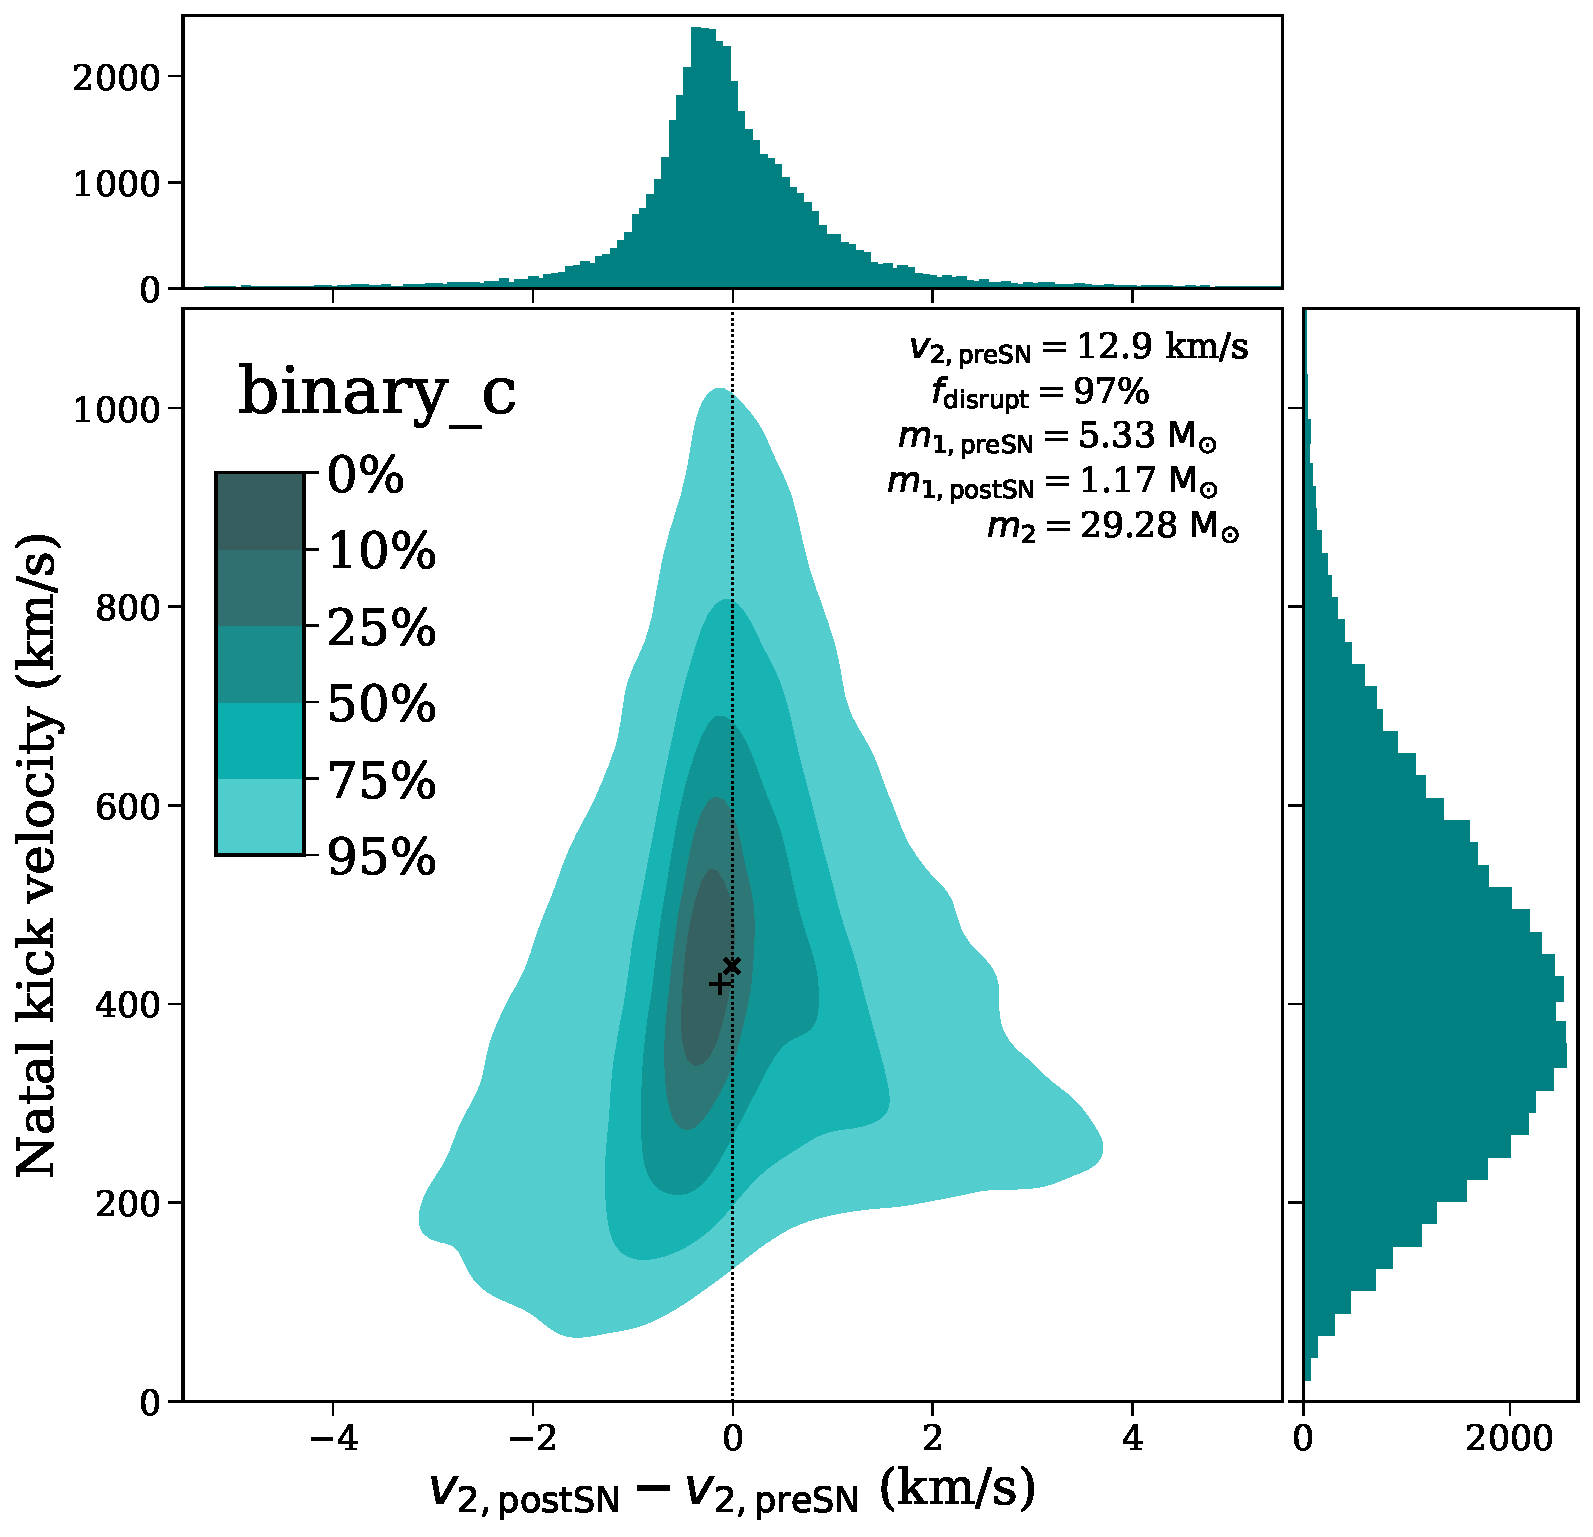
\includegraphics[width=0.45\textwidth]{figures/binary_c.pdf}
    \caption{Secondary ejection velocities closely follow pre-SN orbital velocities, with extremely weak dependence on natal kick magnitudes, across different population synthesis codes. These plots compare a binary with identical initial conditions, evolved 50,000 times with different random natal kicks in three codes. For each code, the main panel shows shows the difference between the secondary ejection velocity and its pre-SN orbital velocity on the $x$-axis, while the $y$-axis shows the natal kick applied to the primary star. Each main panel shows a 2D kernel density estimator with a colourbar indicating the fraction of the population contain with each contour. Secondary panels show marginal histograms. Small black crosses and pluses indicate the mean and median of each distribution respectively. Panels are annotated with the population synthesis code used for evolution and information about the pre- and post-SN system.}
    \label{fig:ejection_vels}
\end{figure*}

The ejection velocities of the secondary star closely follows their pre-SN orbital velocities in each code, and have only a very weak dependence on the magnitude of natal kicks. In Figure~\ref{fig:ejection_vels}, we show how the applied natal kick affects the difference between the pre- and post-SN velocity of the secondary star in these simulations. The main panels show a 2D kernel density estimator for the disrupted binaries in the 50,000 realisations. Quantitatively, we find that, for each code, the ejection velocity of the secondary star is within ${\sim}5\unit{km}{s^{-1}}$ of its pre-SN orbital velocity, despite the natal kick magnitudes spanning 3 orders of magnitude.

The independence of the secondary's ejection velocity and the natal kick applied to the primary is expected. Due to the strength of the natal kicks, the secondary star experiences a near instantaneous disappearance of the compact object from its orbit, removing the centripetal acceleration and leading to its ejection at close to its pre-SN orbital velocity (see \citealt{Tauris+1998:1998AA...330.1047T} for a more in-depth discussion).

The agreement between the codes validates their implementation of the SN kick routines. Although each code produces a markedly different pre-SN evolution of the system (compare the annotations in each plot in Figure~\ref{fig:ejection_vels}), the relationship between the pre- and post-SN velocities holds.

The shape of these distributions can be understood through a consideration of the magnitude and azimuthal angle of the kick, in concert with the geometry of the system. In Figure~\ref{fig:angles}, we show the individual disrupted systems from the \binc simulation as scatter points. As visible in the earlier plots, this distribution narrows towards larger kick values, showing that stronger natal kicks lead to a tighter relationship between the pre- and post-supernova velocities of the secondary star. This tightening is due to the fact that a stronger natal kick more immediately removes the compact object from a system. As a result, the compact object is less able to influence the trajectory of the ejected companion star.

The azimuthal angle of the kick influences the difference between ejection velocity and the pre-supernova velocity of the secondary star. In Figure~\ref{fig:angles}, we include a guide for the geometry of the system in the upper left corner, which shows the direction of ejection of the companion and a coloured wheel indicating the azimuthal angle of the kick. The main plot indicates that the strongest accelerations of the companion occur for angles close to $\omega = 5\pi/6$, while the strongest decelerations occur for angles close to $\omega = \pi/3$. From the geometry of the system, we can see that these angles respectively correspond to a trajectory that leads to the compact object being mostly ahead, or mostly behind, the companion ejection direction. For a compact object that is ahead of the direction of the companion it will increase its velocity, hence the acceleration at these angles, while the inverse reasoning applies for the deceleration. Similarly, natal kicks pointed directly away from the companion ($\omega = 3\pi / 2$) have the weakest effect on the ejection velocity of the companion.

\newpage

For weaker kicks ($\lesssim 250 \unit{km}{s^{-1}}$) the shape of the distribution shifts because the approximation that the compact object near-instantaneously leaves the systems no longer holds. In this regime, a kick directed away from the companion, or behind it's ejection trajectory (i.e.\ $\omega < \pi/2$ or $\omega > 3\pi/2$) can allow the compact object to more significantly decelerate the companion before leaving the system. This is notable in the shift of the distribution to more negative values for weak kicks. Furthermore, a weaker kick with an angle counter to the compact object's orbital motion (i.e.\ $\pi / 2 \le \omega \le 3\pi/2$) can simply decelerate the compact object, tightening the binary, but leaving it bound. This leaves a gap in the distribution of disrupted systems, which we highlight with a grey shaded region. As a results of these effects, the median difference between the pre- and post-SN velocity of the secondary star is negative for weak kicks, as shown by the solid black line in Figure~\ref{fig:angles}.


\begin{figure}
    \centering
    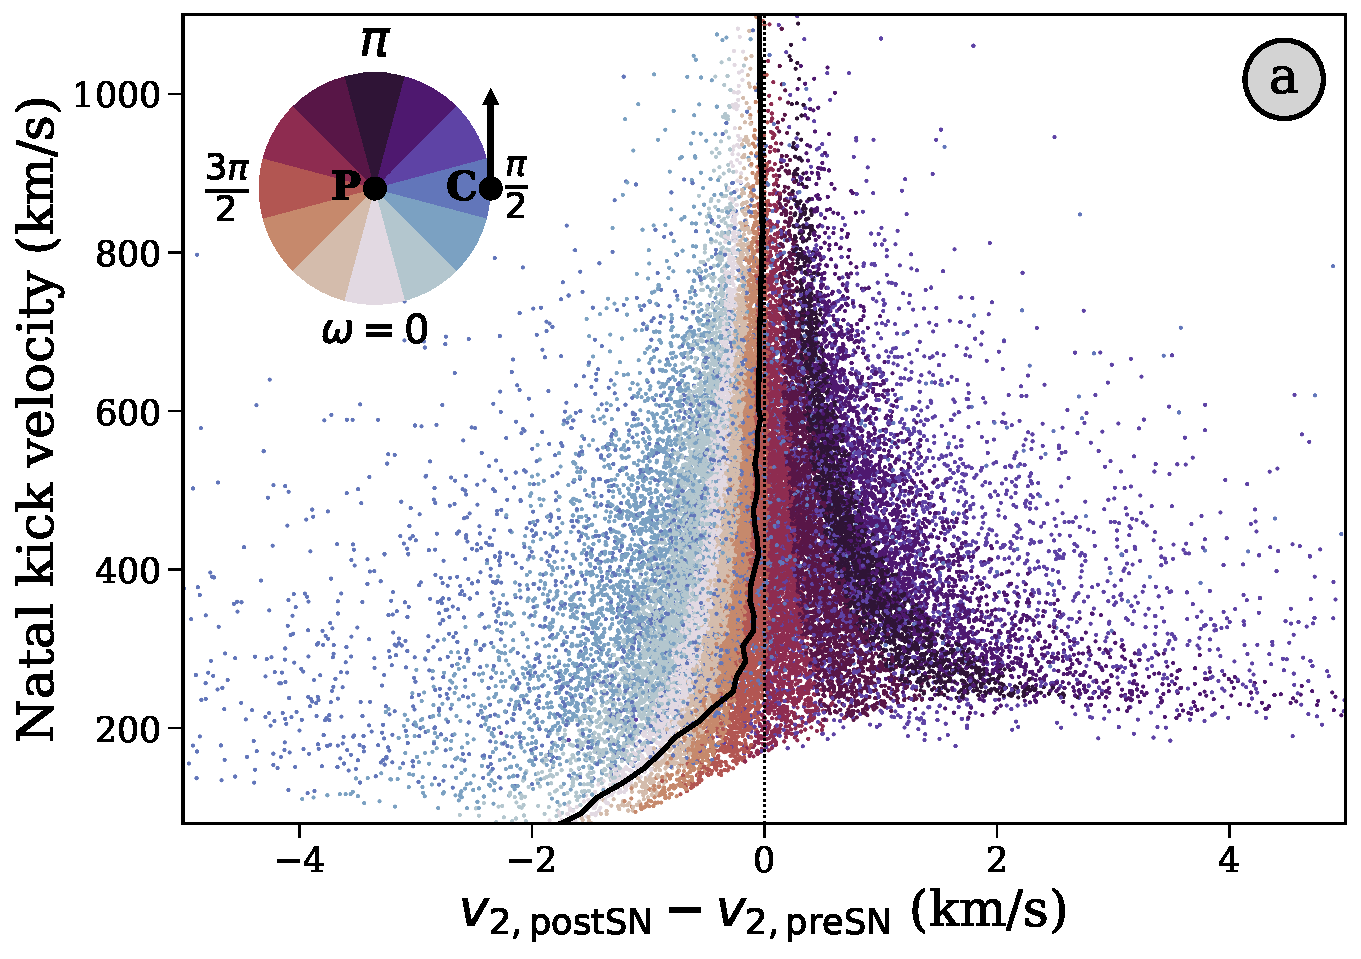
\includegraphics[width=\columnwidth]{figures/binary_c_angles.pdf}
    \caption{The slight variances in the ejection velocity of the secondary star are due to the angle of the natal kick, which are exaggerated for weaker kicks. The scatter points show the 50,000 different realisations of the binary run with \binc, each of which are coloured by the azimuthal angle of the kick. The solid black line shows the median difference between the pre- and post-SN velocity of the secondary star as a function of the natal kick magnitude. In the upper left corner we include a guide for the geometry of the system, where P is the primary (exploding) star, C is the (ejected) companion star, the arrow indicates the pre-SN orbital velocity of the companion and the wheel of colour indicates the azimuthal angle of the natal kick. The shaded region in the lower right indicates where systems remain bound for weak natal kicks that send the compact object in a similar direction as the companion.}
    \label{fig:angles}
\end{figure}

\section{Correction to Kiel \& Hurley (2009)}\label{sec:kiel}

Earlier versions of \cosmic ($<$v3.5.0) used the methodology described by \citet{Kiel+2009:2009MNRAS.395.2326K}, hereafter \citetalias{Kiel+2009:2009MNRAS.395.2326K}, in calculating the post-SN orbital properties of binaries, as well as the ejection velocities of compact objects and their prior companions. However, when using this method, we found that the ejection velocities of companions were not strongly correlated with their pre-SN orbital velocities as one would expect. Instead, their ejection velocity showed an (unphysical) strong dependence on the natal kick received by the primary. Moreover, the ejection velocity of the compact object was often significantly slower than the natal kick that it received.

We demonstrate the strong dependence of the ejection velocity on natal kick magnitude in Figure~\ref{fig:kiel_comparison}. The grey contour plot shows the distribution of ejection velocities and natal kick magnitudes for our representative binary evolved 50,000 times with the original \citetalias{Kiel+2009:2009MNRAS.395.2326K} prescription. The triangular shape of the contour indicates that stronger natal kicks also lead to faster ejection velocities. Moreover, the marginal distribution in the upper panel of Figure~\ref{fig:kiel_comparison} shows there is a wide spread in ejection velocities, extending up to 4 times the pre-supernova orbital velocity. This is unphysical, as the ejection velocity of the companion should be closely related to its pre-SN orbital velocity.

\begin{figure}
    \centering
    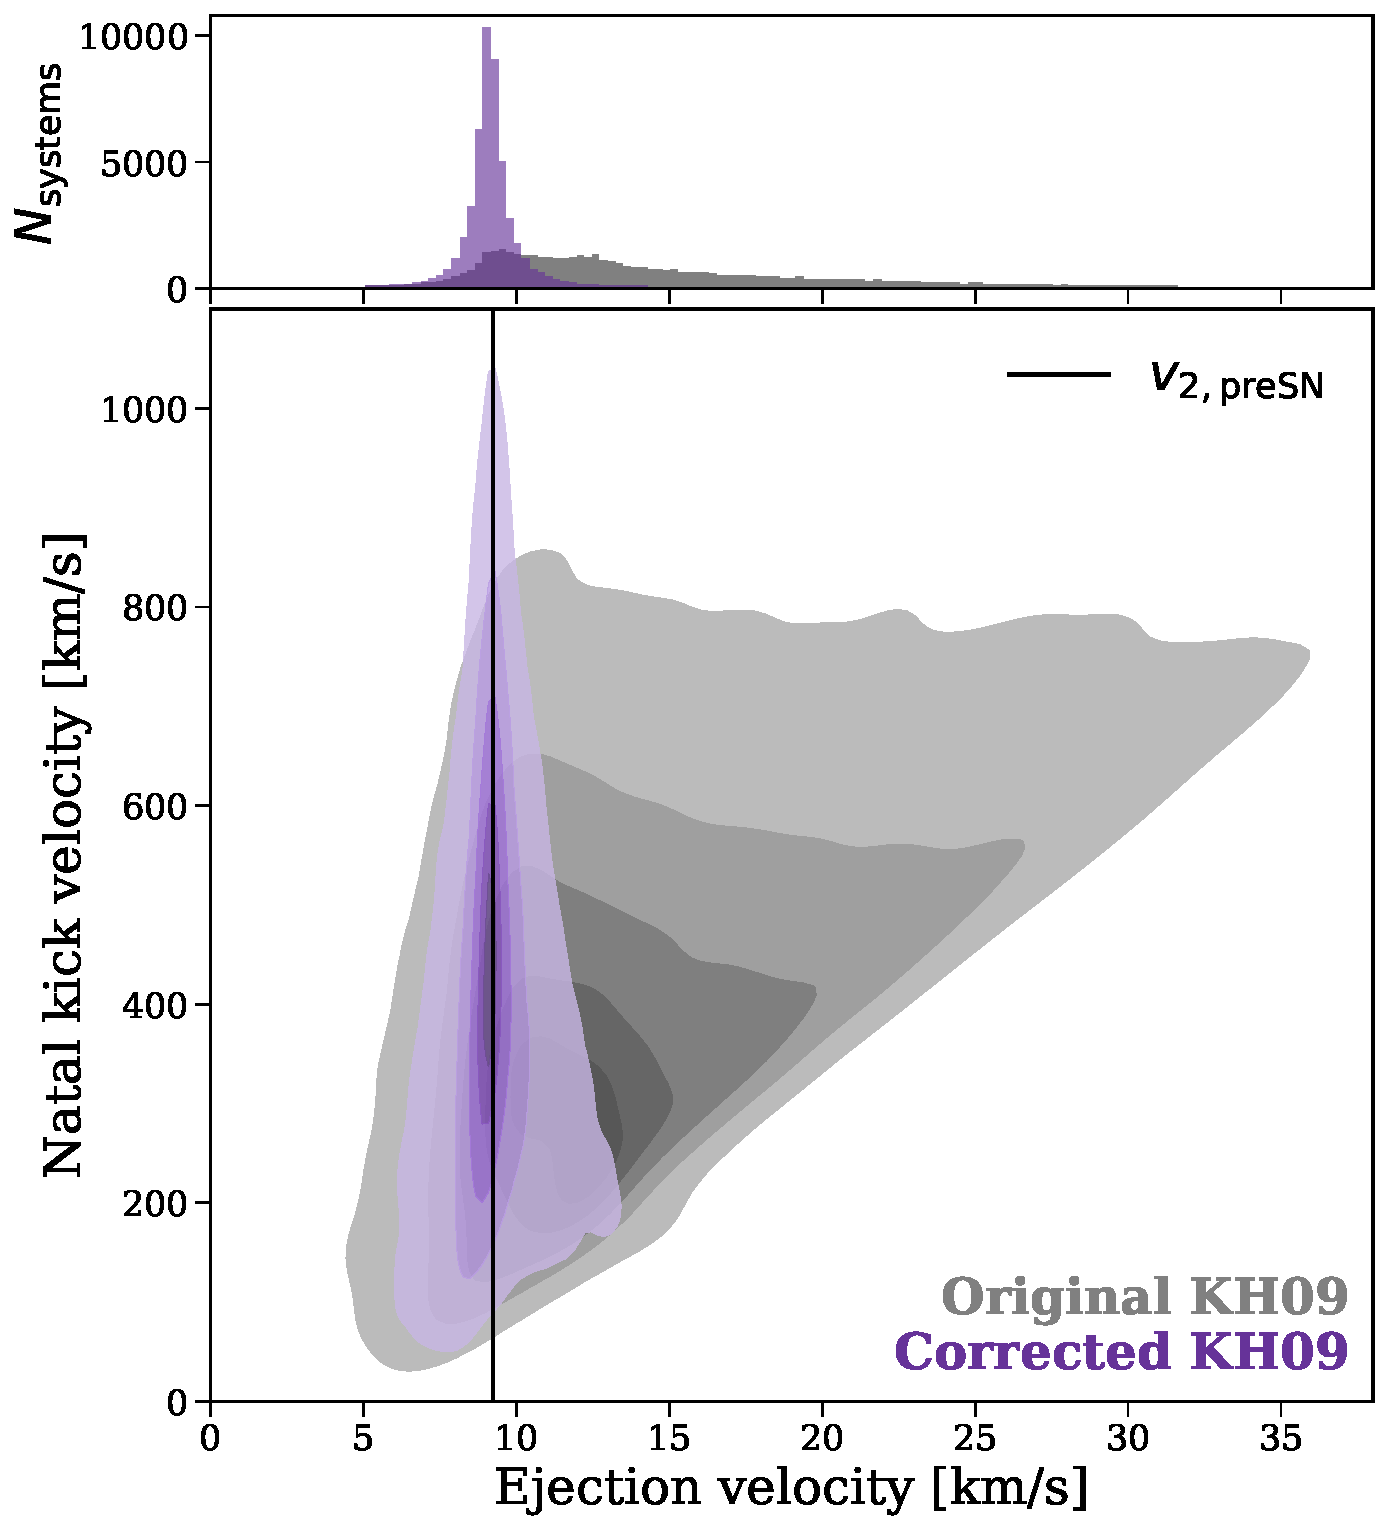
\includegraphics[width=\columnwidth]{figures/cosmic_kiel_comparison.pdf}
    \caption{Our correction to \citet{Kiel+2009:2009MNRAS.395.2326K} removes an unphysical dependence of the ejection velocity of secondary stars on the magnitude of the primary star's natal kick. The main panel shows kernel density estimators for the 2D density distributions, with and without our correction. The upper panel shows the marginal distribution for the ejection velocity.}
    \label{fig:kiel_comparison}
\end{figure}

The reason for these effects is that, in \citetalias{Kiel+2009:2009MNRAS.395.2326K}, the $z$ component of the final velocity of each binary constituent neglects the contributions from the velocity at infinity of the hyperbolic orbit, $V_\infty$. The derivation assumes that this velocity is directed entirely within the orbital plane of the binary, but does not fully account for the fact that the orbital plane is no longer aligned with the $z$ axis after the SN. Therefore, the $z$ component of the final velocity of the compact object (equation 17 from \citetalias{Kiel+2009:2009MNRAS.395.2326K}) should be as follows
\begin{equation}
    V_{\rm 1fz} = \frac{M_{\rm NS}}{M_b^{\prime}} V_{\rm kick} \sin \phi + V_{\infty} \sin \nu \sin \gamma \frac{M_2}{M_b^\prime},
\end{equation}
where the variables are defined in the same way as \citetalias{Kiel+2009:2009MNRAS.395.2326K}, such that $M_{\rm NS}$ is the mass of the resulting compact object, $M_b^\prime$ is the final total mass of the system, $V_{\rm kick}$ is the magnitude of natal kick, $\phi$ is the polar angle of the natal kick, $V_\infty$ is the velocity at infinity of the hyperbolic orbit and $\nu$ and $\gamma$ are angles accounting for the misalignment of the orbital plane after the SN (see Section 2.2.1 and Figure 2 of \citetalias{Kiel+2009:2009MNRAS.395.2326K}). Similarly the $z$ component of the final velocity of the companion (equation 20 from \citetalias{Kiel+2009:2009MNRAS.395.2326K}) should be as follows
\begin{equation}
    V_{\rm 2fz} = \frac{M_{\rm NS}}{M_b^{\prime}} V_{\rm kick} \sin \phi - V_{\infty} \sin \nu \sin \gamma \frac{M_{\rm NS}}{M_b^\prime}.
\end{equation}

We have confirmed that the inclusion of the additional $V_\infty$ terms in these equations removes the unphysical dependence on natal kick magnitude. In Figure~\ref{fig:kiel_comparison}, the purple distributions correspond to the corrected version of \citetalias{Kiel+2009:2009MNRAS.395.2326K}, which now strongly correlates with the pre-supernova orbital velocity. This brings the \citetalias{Kiel+2009:2009MNRAS.395.2326K} method into agreement with that of \citet{Pfahl+2002} and \citet{Tauris+1998:1998AA...330.1047T}.

The latest versions of \cosmic ($\ge$v3.5.0) now use the \citet{Pfahl+2002} method by default. We make the original \citet{Kiel+2009:2009MNRAS.395.2326K} method accessible (via negative \texttt{kickflag} inputs) so that earlier \cosmic results can be reproduced. We note that this issue only affected the ejection velocities of stars and compact objects from disrupted systems, but the \textit{conditions} for disruption and post-SN orbital parameters for \textit{bound} systems were correct. Therefore prior work using \cosmic to explore bound systems remains unchanged.

\section{Code issues identified and resolved as a result of comparison}

During the course of this comparison we identified problems with either the kick prescription or implementation in each of the codes that we considered.

As discussed above, \cosmic previously used an erroneous kick prescription, which has been resolved as of v3.5.0\footnote{\url{https://github.com/COSMIC-PopSynth/COSMIC/pull/678}}. The implementation in \compas had anomalous component velocities such that the ejection velocity of secondary stars was consistently overestimated by a factor of 2. This problem arose as a result of spurious vector indexing and incorrect rotation algebra in the code. This issue has been resolved as of \compas v03.09.02\footnote{\url{https://github.com/TeamCOMPAS/COMPAS/pull/1290}}. In \binc, the prior implementation did not sample natal kick magnitudes and azimuthal angles in an independent manner, which led to slightly lower ejection velocities on average. This correlated sampling occurred as a result of re-using a randomly generated number from the kick magnitude in the azimuthal angle sampling. This issue has been resolved as of \binc vX.X.X \footnote{\url{https://gitlab.com/binary_c/binary_c/-/commit/fba20687984e9cfb46bc38838d07655bfc99c6e5}}.\david{What version should I write here?}

Despite the rigorous testing suites of each code that aim to address issues such as these, each bug was not uncovered until comparison with other open-source codes. This highlights the fact that open-science, and comparison projects such as these, are essential to identifying and resolving subtle issues in population synthesis.

\section*{Acknowledgements}
We thank Eric Bellm and Andy Tzanidakis for helpful discussions. TW and KB acknowledge support from NASA ATP grant 80NSSC24K0768.

\textit{Software:} This work made use of the following software packages: \texttt{astropy} \citep{astropy:2013, astropy:2018, astropy:2022}, \texttt{Jupyter} \citep{2007CSE.....9c..21P, kluyver2016jupyter}, \texttt{matplotlib} \citep{Hunter:2007}, \texttt{numpy} \citep{numpy}, \texttt{pandas} \citep{mckinney-proc-scipy-2010, pandas_13819579}, \texttt{python} \citep{python}, \texttt{scipy} \citep{2020SciPy-NMeth, scipy_13352243}, \texttt{COSMIC} \citep{Breivik2020, COSMIC_13854578}, \texttt{Cython} \citep{cython:2011}, \texttt{h5py} \citep{collette_python_hdf5_2014, h5py_7560547}, \texttt{schwimmbad} \citep{schwimmbad}, \texttt{seaborn} \citep{Waskom2021}, and \texttt{tqdm} \citep{tqdm_13207611}. This research has made use of NASA's Astrophysics Data System. Simulations in this paper made use of the COMPAS rapid binary population synthesis code (version 3.01.10), which is freely available at \url{http://github.com/TeamCOMPAS/COMPAS} \citep{COMPAS}. Software citation information aggregated using \texttt{\href{https://www.tomwagg.com/software-citation-station/}{The Software Citation Station}} \citep{software-citation-station-paper, software-citation-station-zenodo}.

\newpage

\bibliographystyle{aasjournal}
\bibliography{main}{}

\end{document}